% !TeX root = ../main.tex

\chapter{Experiments and Evaluation}\label{chapter:Evaluation}

The evaluation focuses on measuring the model’s effectiveness in meeting the stated objectives as defined in Chapter~\ref{chapter:introduction}.
In particular, it examines the reduced scheduling latency and kernel overhead when invoking kernel functions.
The results highlight both the benefits of the approach and its limitations.


\section{Limitation in Memory Transfers during Evaluation}

During testing, the evaluation revealed nondeterministic behavior in the execution results.
In some runs, the kernels scheduled did not use the correct input matrices but instead used uninitialized memory, resulting in output matrices containing only zeros.
Under further testing, this issue never occurred when debugging print statements were inserted, suggesting that the nondeterministic issue was timing-related.
In particular, the input arguments were being processed before they were available. 
While this issue was not addressed in the current implementation, documenting it is important to understand the limitations and potential challenges associated with using persistent GPU threads for real-time workloads.

Given that the print statements ensured correct execution and the values inside the kernel functions were observed to be incorrect, the issue lies with the enqueuing of tasks to the GPU. 
The task enqueuing process first copies memory, then copies the task into the respective buffers within the same stream, and only afterward notifies the GPU of the new functions.
Therefore, the memory should be consistent and correct before the task is even in the buffer to be executed. 
However, the GPU periodically polls for new tasks after a deadline to avoid missing updates if the CPU enqueues a task while the message flag is reset.
When this polling occurs as the task is being copied into the memory buffer, it is possible that a memory copy is completed only partially, resulting in correct execution values but an incorrect offset. This can lead to incomplete or invalid matrices being processed.

This hypothesis remains unproven; however, in cases with incorrect values, kernel execution times are significantly reduced, which can lead to incomplete analysis of the results. 
Therefore, the evaluation in the following graphs contains only the execution runs that correctly computed all values within the task queue.

\section{Experimental Setup}

To assess the effectiveness of persistent threads in reducing scheduling latency, the solution was tested against a baseline implementation using a matrix multiplication benchmark. 
For this analysis, a simple random matrix multiplication task was repeatedly generated and scheduled 32 times using the persistent thread implementation.
The measured latency was then compared to a straightforward kernel invocation. 
All experiments were conducted on an NVIDIA Tesla V100 GPU running CUDA version 11.8.

\subsection{Matrix Multiplications for Performance Testing}

The current execution model requires manual task wrappers for scheduling and executing GPU tasks, which adds complexity when supporting a variety of functions. 
These wrappers reduce the overhead of GPU memory allocation, but require serialization and deserialization of the data during execution.
To keep testing manageable, this thesis focuses on matrix multiplications as a representative example to demonstrate the solution's capabilities. 

In particular, the benchmark uses matrix multiplications of a fixed size, 16 x 16, chosen due to the inflexibility of changing configurations during the kernel's lifetime. 
Typically, the programmer specifies kernel thread configurations at launch; however, this is not possible with persistent threads.
Their configuration is fixed at launch and cannot be changed during execution.
In practice, such values need to be determined by profiling the workload and implementing them manually.
Since performance improves when the number of threads matches or exceeds the number of elements in the solution matrix, this implementation uses a 16×16 matrix with a 16×16 grid dimensionality.

\subsection{Simulated Workload for Testing}

Because the benchmark and persistent kernel implementations differ in their application goals, a simulated workload was designed for testing purposes. 
In these tests, the persistent kernel task schedules 32 random matrix multiplication tasks to the GPU and then immediately begins waiting for results. 
As the tasks are being scheduled, the GPU concurrently executes already enqueued tasks. 
After completing individual tasks, the host is notified via the mailbox message. 
By contrast, the matrix multiplication benchmark executes tasks serially in an allocation, memory copy, kernel launch, and memory copy back loop.  


\subsection{Latency Measurements}


\begin{figure}[H]
  \centering
  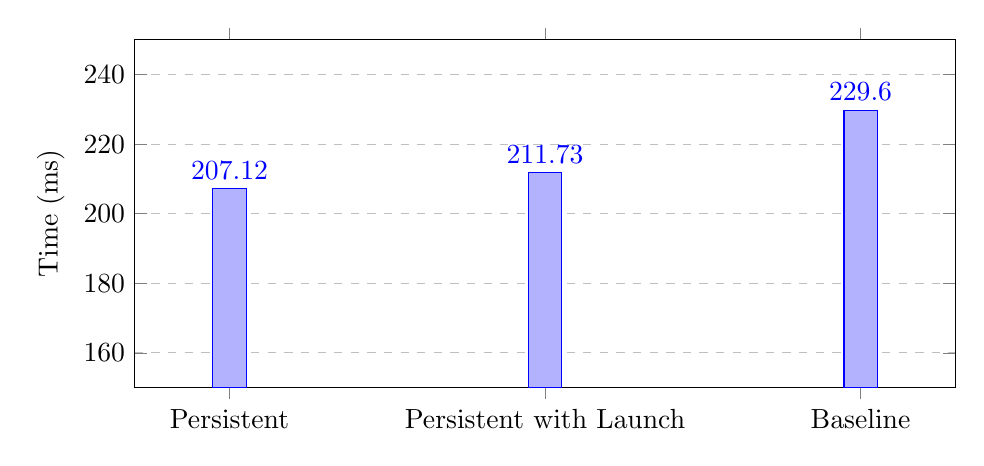
\begin{tikzpicture}
  \begin{axis}[
    ybar,
    bar width=12pt,
    width=12cm,
    height=6cm,
    ymin=150,
    ymax=250,
    ylabel={Time (ms)},
    symbolic x coords={{Persistent}, {Persistent with Launch}, {Baseline}},
    xtick=data,
    nodes near coords,
    nodes near coords align={vertical},
    enlarge x limits=0.15,   % tighter horizontal spacing
    ymajorgrids=true,        % light grid lines for readability
    grid style=dashed,
  ]
    \addplot coordinates {({Persistent}, 207.121) ({Persistent with Launch}, 211.727) ({Baseline}, 229.604)};
  \end{axis}
\end{tikzpicture}


  \caption{Small Kernel and Memory Transfer Tasks}
  \label{fig:sm_sk}
\end{figure}


Figure~\ref{fig:sm_sk} presents the first experiment, comparing task scheduling using the GPU persistent kernel against the baseline model. 
Here, each implementation executes 32 tasks of 16x16 matrix multiplication tasks scheduled to the GPU. 
The matrices for testing are generated at runtime and compared to the correct CPU implementation using the same functions.  

Across 10,000 runs, the persistent kernel achieved an execution time of 207.12 ms, compared to 229.60 ms for the baseline model. 
This demonstrates a clear performance advantage for the persistent kernel in cases where small kernels are used with modest memory transfers. 
However, the measurements exhibited high variability, with execution times differing by as much as $\pm$50 ms between runs, even when averaged over 10,000 executions.
Despite this variability, the persistent kernel consistently outperformed the baseline in trials.


\subsection{Latency Measurements with large Memory Transfers}

\begin{figure}[H]
  \centering
  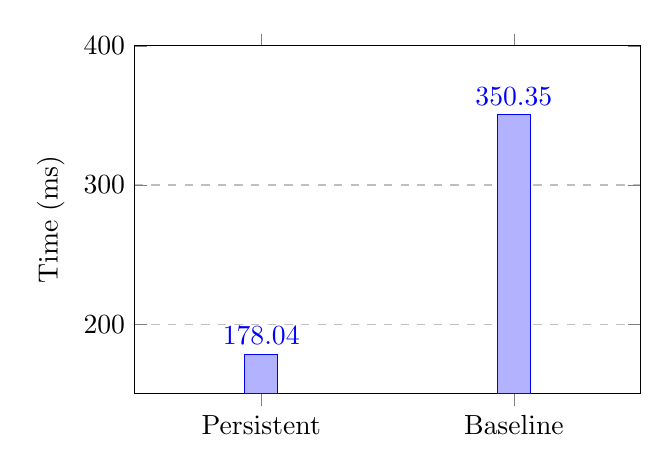
\begin{tikzpicture}
  \begin{axis}[
    ybar,
    bar width=12pt,
    width=8cm,
    height=6cm,
    ymin=150,
    ymax=400,
    ylabel={Time (ms)},
    symbolic x coords={{Persistent}, {Baseline}},
    xtick=data,
    nodes near coords,
    nodes near coords align={vertical},
    enlarge x limits=0.50,   % tighter horizontal spacing
    ymajorgrids=true,        % light grid lines for readability
    grid style=dashed,
  ]
\addplot coordinates {(Persistent, 178.035) (Baseline, 350.349)};
  \end{axis}
\end{tikzpicture}

  \caption{Small Kernel and Larger Memory Transfer Tasks}
  \label{fig:bm_sk}
\end{figure}

In this secondary evaluation, the GPU executes the same task as before but with an additional 1 MiB of memory transferred to and from each task.
Interestingly, the persistent thread implementation ran slightly faster than in the previous test, while the baseline control became significantly slower.
For reference, the persistent kernel completed in 178 ms, compared to 350 ms for the non-persistent version.
This unexpected outcome prompted further testing with a larger input size of 10 MiB, which completed in 623.915ms.

The performance improvement is likely attributable to the underlying memory management strategy. 
To conserve GPU resources, memory buffers are partitioned logically using offsets.
When tasks use very small memory frames, their data is placed closely together in memory.
During execution, this proximity can lead to contention: tasks from memory locations adjacent to those being written to by other tasks may experience reduced performance.
By increasing the memory size transferred per task, the allocated regions are spaced farther apart, reducing contention and allowing the kernel to execute more efficiently.

\section{Multiple GPU Blocks}

Unfortunately, particularly in the case of running multiple GPU blocks, the memory copying errors were observed with a much higher frequency. 
As the GPU blocks were polling more frequently and able to consume tasks more quickly, they had faulty, uninitialized parameters.  
The results from this test failed too often to support any claims. 


\chapter{Conclusion and Future Work}


This work presents a GPU persistent thread model, designed both as a foundation for future research in scheduling and as a way to improve the efficiency of executing multiple tasks on the GPU by reducing kernel launch overhead.
The model supports application-specific fine-tuning, with particular focus on managing hardware resources.
In this approach, the persistent kernel runs throughout the application's lifetime, dynamically processing incoming tasks streamed to the GPU and avoiding repeated kernel launches.

The implementation meets the objectives established for developing a real-time GPU scheduler.
In particular, it demonstrates that persistent threads reduce scheduling overhead and improve latency. 
Furthermore, Chapter~\ref{chapter:Persistent Threads}  outlines how priorities and coroutines could be integrated into this persistent thread model. 
Overall, this work enhances understanding of real-time GPU scheduling, CUDA architecture, and GPU execution and programming models, providing a foundation for future improvements and research in high-performance real-time GPU computing.

\section{Limitations and Future Work}

The primary limitation observed is the non-deterministic results discussed in Chapter~\ref{chapter:Evaluation}. 
This behavior arises from the way tasks are enqueued.
While the GPU should manage tasks to provide support for fine-grained scheduling, it must also ensure data consistency.
In this implementation, the GPU needs to decouple memory transfers and context information from the actual execution logic.
Once the transfer and context information has been transferred, then the action can be executed. 

This could be addressed in several ways to synchronize the GPU with the CPU further.
Currently, the synchronization mechanism of GPU mailboxes only supports a single mailbox. 
Instead, the implementation could support a mailbox per task element or one per \acs{SM}, allowing GPU \acs{CTA} blocks to constantly synchronize on these tasks, rather than on the tail of the queue. 
Furthermore, this approach enables the GPU to assign tasks to specific partitions, thereby reducing interference. 
Another approach is to introduce a separate execution buffer that only allows task execution after all necessary data has been copied and made stream-coherent.
Lastly, the GPU could track the number of tasks waiting for execution using a synchronization method, which is only updated after tasks are coherent. 

Additional limitations include the manually written wrappers used for serializing and deserializing parameters.
These wrappers introduce extra overhead and complexity for the user, making the system slower and more labor-intensive than an automatic solution would be.
Addressing these limitations represents a clear path for future work to support reliable, efficient, and user-friendly persistent thread-based scheduling.

\section{Future Work}
The current system does not support priority-based scheduling decisions or the use of coroutines for software preemption execution.
Future work could build on the strategies outlined in this thesis to utilize the persistent kernel implementation as a foundation for these features, enabling more predictable real-time scheduling. 
In this case, the memory management system may need to transition from an epoch-based scheduler to a more complex management system. 
Additionally, the current manual streaming of input and output parameters limits task variability and automation.  
Developing a generalized parameter serialization and deserialization layer that supports arbitrary kernel arguments would increase flexibility and reduce overhead in task preparation.

Two particularly promising directions for GPU persistent threads are GPU partitioning and automatic task generation through interception.
By fully allocating GPU resources and using PTX code to define the behavior of individual \acs{SM}s, persistent threads can enforce manual GPU partitioning, reducing interference between tasks. 
Additionally, implementing a CUDA API interception to capture and schedule tasks automatically would significantly enhance both the implementation of persistent threads in other projects and the ease of adapting these tasks to new workloads.

\section{Conclusion}

Overall, while the current implementation demonstrates the feasibility of persistent GPU threads, it remains a relatively more straightforward exploration of the concept.
There is substantial opportunity for further optimization, refinement, and scaling to unlock the full potential of this approach and incorporate additional real-time scheduling strategies into the framework.
Future work could build on this foundation to develop more sophisticated scheduling strategies, enhance automation, and provide better support for complex real-time workloads.


%If too many tasks are scheduled or the memory buffer becomes fully saturated, task enqueueing fails and the launch function returns a \texttt{-1} error code.  
%Therefore, proper usage requires either a fault-tolerant launching mechanism that can handle task rejections or a carefully designed launch strategy to avoid buffer overflow.




